\section{Results and Discussion}

To give a flavour of the protocols we explore in this thesis, we present here
an overview of our NIPoPoW protocol, which sits at the heart of proof-of-work
blockchain interoperability.

A simplified description of our NIPoPoW protocol is as follows. Initially, some value
$m$ is fixed, representing the number of blocks that the verifier wishes to
receive to feel safe. This $m$ is a constant parameter. The honest prover then
chooses the highest level $\mu$ which has at least $m$ blocks at that level.
Choosing any level above $\mu$ would not satisfy the verifier, as fewer than $m$
blocks would be transmitted. Choosing any level below $m$ would be wasteful, as
more blocks would have to be transmitted. This prover choice is illustrated in
Figure~\ref{fig.level-threshold}. Suppose that the verifier receives two
proofs from two provers, one of which is honest while the other adversarial, and
wishes to compare them. The verifier first checks that all the blocks it has
received really are $\mu$-superblocks by verifying the proof-of-work equation
parameterized by $\mu$ is satisfied, and that each proof it has received has at
least $m$ blocks. Then, just as a full verifier would compare the length of two
full chains, the NIPoPoW verifier now simply \emph{counts} the number of blocks
it has received from the two provers and announces that the one with the most
blocks is the winner. If the verifier receives the proofs $\pi_1$ and $\pi_2$,
then the decision is simply the result of the comparison $|\pi_1| > |\pi_2|$.

\begin{figure}[ht]
    \caption{A superblock NIPoPoW prover chooses the threshold (dashed line)
    corresponding to level $\mu = 2$ for the verifier requirement $m = 4$.}
    \centering
    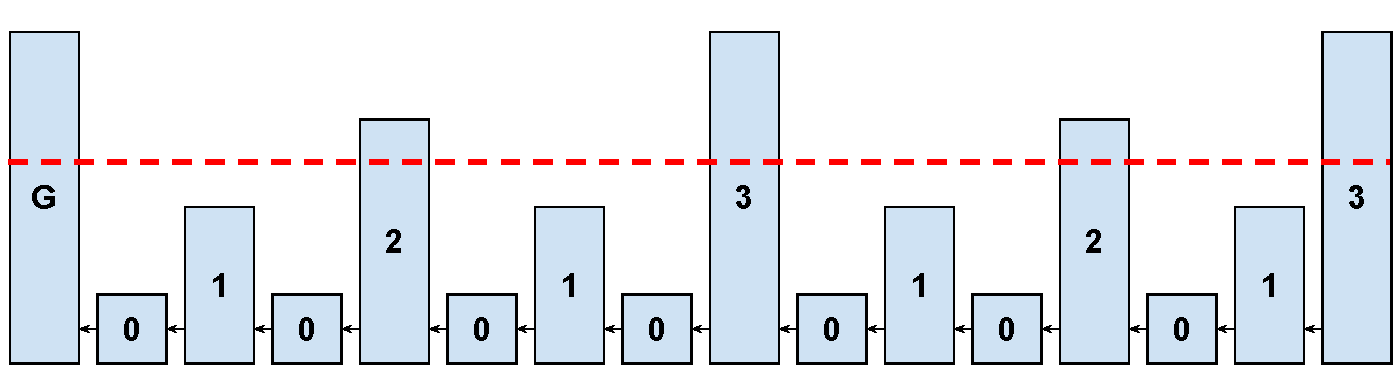
\includegraphics[width=0.7\columnwidth,keepaspectratio]{../chapters/introduction/figures/level-threshold.pdf}
    \label{fig.level-threshold}
\end{figure}

The crucial point in terms of security is that an adversary cannot fake this
set of superblocks without actually putting in the work. An adversary that
produces a $\mu$-superblock will also in expectation generate some $2^\mu$
regular blocks in the process (even though the adversary may of course choose
to discard these). Because the adversary has minority mining power, an adversary
cannot create a longer sequence of $\mu$-superblocks faster than the honest
parties create one, for the same reason that an adversary cannot create a longer
regular blockchain faster than the honest parties create one.

Let us count how many different levels $\mu$ there are in a chain. If the chain
has length $|\chain|$, then going up to level $1$ cuts the chain in half, and we
expect to see only $\frac{|\chain|}{2}$ superblocks of level $1$. Moreover, this
continues with subsequent increases in level, until at level $\mu =
\log|\chain|$ we expect to find only $\frac{|\chain|}{2^\mu} = 1$ block. As soon
as we get to level $\log|\chain| + 1$, we expect to find no more blocks of that
level or above. The number of levels is therefore $\log|\chain|$.

To ensure that the blocks sent by the prover cannot be reordered in the wrong
chronological order, just as in the regular underlying blockchain, we need to
introduce pointers that point between consecutive blocks of the same level. As
such, a $\mu$-superblock must include in its contents a pointer to the most
recent $\mu$-superblock that was mined before it. Unfortunately, we cannot add
just these exact pointers to the block contents, because the pointer data must
be included in the contents that are hashed during the attempt to find
proof-of-work. It seems that we must predict what level a block will have prior
to it being mined, but its level depends on its hash, which is a product of its
mining. Therefore, we will simply include all the pointers that could be needed
regardless of what level the block achieves. Prior to mining any block, the
miner collects a pointer to the most recent superblock of each level it has seen
so far. It places these pointers in a list which it then includes in the block
it is mining. When the block is mined, regardless of what level it achieves, it
will have a pointer to the most recent block of its own level.

The number of pointers that need to be included in this manner is small because
the number of levels the blockchain will ever reach is $\log|\chain|$. This
interlinking is illustrated in Figure~\ref{fig.hierarchy4}. To avoid premining of
superblocks (blocks that were mined prior to the creation of the genesis block),
we require that the interlink vector of every block also contains a pointer to
the genesis block. By having miners add these extra pointers to blocks, the
verifier can check that the blocks in each proof presented have been mined in
the order given. We see that NIPoPoWs are \emph{subchains} of the blockchain in
that they form subsequences of the block sequence and also maintain pointers
across. The change of adding interlink pointers seems on the surface to require
that miners change their behavior and so a hard fork (a breaking change of
consensus protocol rules) is required. However, the upgrade can be deployed
using a soft fork (a backwards-compatible change), or even without requiring any
miner upgrade in what we introduce as a \emph{velvet fork}.

\begin{figure}[ht]
    \caption{The interlinked blockchain. Each superblock is drawn taller
    according to its level. A new block links to all previous blocks that
    have not been overshadowed by higher levels in the meantime.}
    \centering
    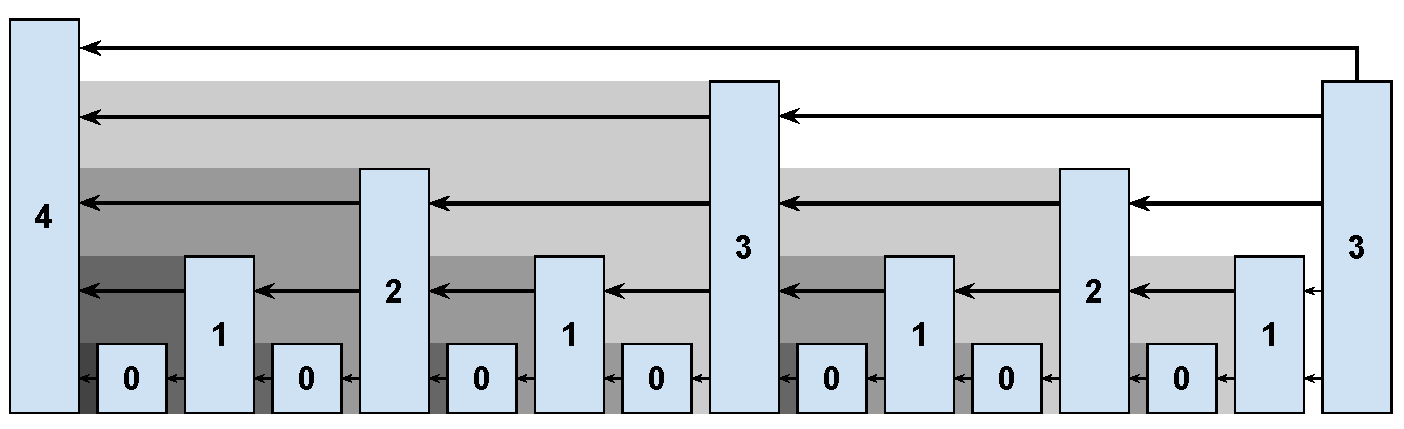
\includegraphics[width=0.9\columnwidth,keepaspectratio]{../chapters/introduction/figures/level-shadows.pdf}
    \label{fig.hierarchy4}
\end{figure}

Because the two provers may send chains of different levels, it may be necessary
for the verifier to compare the two proofs according to different levels. For
this purpose, the verifier weights the proofs according to their level prior to
comparison. The result of the comparison is then
$2^{\mu_1}|\pi_1| > 2^{\mu_2}|\pi_2|$, where $\mu_1$ and $\mu_2$ indicate the
level of proofs $\pi_1$ and $\pi_2$ respectively. If the two proofs are at the
same level, this comparison reduces to a simple comparison by count.

\subsection{Comparing NIPoPoWs}
While the protocol we have presented so far works \emph{in expectation} against
any adversary, we want to design a protocol that also works \emph{with
overwhelming probability}.  Let us now discuss the role of the security
parameter $m$ that the verifier requires for safety. The property we can prove
from the honest majority assumption is that, in a given period of time that is
sufficiently long, the honest miners mining on their regular $0$-level chain
will generate more $\mu$-superblocks than an adversary with any mining strategy.
This ``sufficiently long'' period of time is ensured by the $m$ security
parameter that the verifier requires. If any of the two superchains consists of
at least $m$ superblocks, this must necessarily have required a long time to
generate as long as $m$ is sufficiently large (this can be
made precise with a Negative Binomial Chernoff bound). If a sufficiently long
time has passed, the length of the superchains will be close to their
expectations and correspond to the mining power of the adversary and the honest
parties respectively (this can be made precise with a Binomial Chernoff
bound). Because the adversary has minority mining power, her superchain will
be shorter with overwhelming probability. As we increase the parameter $m$ to
some reasonable value (say $m = 128$), the probability that an adversary is able
to attack our protocol drops exponentially in $m$ (according to a function
asymptotically similar to $2^{-m}$).

If the honest and adversarial verifiers send chains that share some blocks,
there is some probability that the adversary is able to convince an honest
verifier of an invalid claim. What we wish to ensure is that the honest NIPoPoW
verifier will never be made to disagree with a corresponding full verifier. For
the argument outlined above to hold, we must ensure that the verifier requests
from the two provers at least $m$ superblocks that are \emph{distinct} in each
of their proofs. This ensures the adversary will not be able to reuse blocks
from the honest chain in her proof. Towards this purpose, the verifier asks the
two provers to choose a level $\mu$ such that there are at least $m$ blocks in
each of their proofs \emph{after} the most recent block shared among their
chains (the \emph{lowest common ancestor block} or \emph{LCA block}) as
illustrated in Figure~\ref{fig.lca-comparison}.

\begin{figure}[ht]
    \caption{A comparison across two chains sharing an LCA. The comparison must
    be performed on the independent subchain suffixes after the highlighted block.}
    \centering
    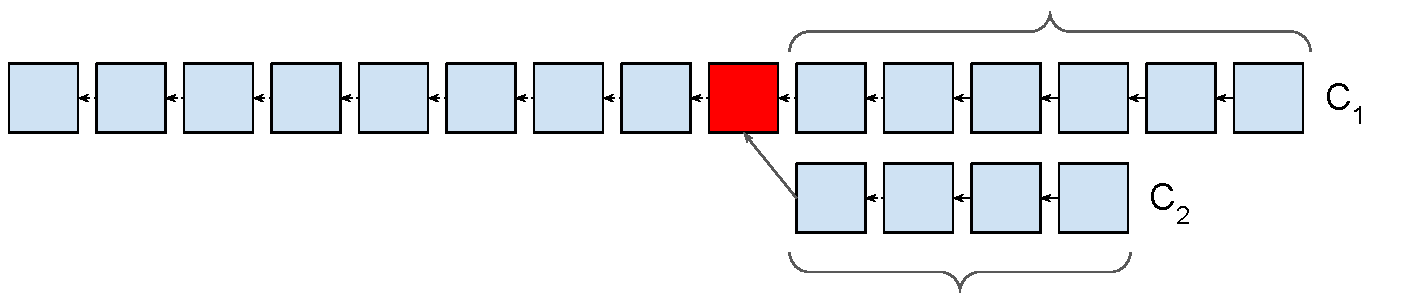
\includegraphics[width=0.9\columnwidth,keepaspectratio]{../chapters/introduction/figures/lca-comparison.pdf}
    \label{fig.lca-comparison}
\end{figure}

This can be solved by introducing interactivity in a protocol that works as
follows. Initially, both provers send their highest level $\mu$ that has at
least $m$ blocks to the verifier. The verifier inspects both proofs and finds
their LCA block $b$. He then sends the LCA back to the provers and requests more
information. Each prover subsequently finds the highest level $\mu'$ that has at
least $m$ blocks \emph{after block} $b$. He sends all blocks of level $\mu'$ that
follow $b$. The verifier again inspects the two
proofs and finds their new LCA block $b'$. The process continues until one of the
two provers is not able to keep up with the interrogation. The number of
interrogation steps will be logarithmic, as they are bounded by the number of
levels. Because there can be
no two chains at level $0$ which are both long and significantly diverge, one of
the two provers will necessarily fail.

While it seems that this requires some interactivity, in reality the provers can
provide sufficient evidence upfront so that no interrogation is needed and the verifier can compare proofs
completely
offline. The prover must ensure that there are sufficient blocks in the proof to
enable a comparison regardless of which block is deemed to be the LCA block (as
the adversary can create a proof which essentially chooses the LCA in her
favour). As such, no matter what block in his proof is chosen as the LCA block
$b$ after which the comparison will be performed, the honest prover wants to
ensure he will be successful. The prover includes sufficient blocks so that for
every block $b$ in his proof (a candidate LCA), there exists some level $\mu$
for which at least $m$ superblocks of that level will appear after $b$.
Furthermore, to ensure no work is missed, the honest prover wants \emph{all} his
blocks of the chosen level to appear after $b$.

This requires us to build a prover that sends blocks at multiple levels. A
summary of the construction is then as follows. The prover first chooses the
highest level $\mu$ which has at least $m$ blocks. He sends all
$\mu$-superblocks. Then, for each lower level $j - 1$, he sends sufficient
blocks of level $j - 1$ to cover the same range that the last $m$ blocks of level
$j$ span. The blocks that are selected for sending in such a NIPoPoW are
illustrated in Figure~\ref{fig.nipopow-example}. In this example, the protocol is
working with parameter $m = 3$. Initially, the prover chooses the \emph{highest}
level $\mu$ that has at least $m = 3$ blocks. In this case, he selects $\mu = 2$
which has $4 \geq m$ blocks, as level $3$ would be insufficient with only $2 <
m$ blocks. All $4$ blocks of $\mu = 2$ are included. Subsequently, the last
$m = 3$ blocks of level $\mu = 2$ are considered and the $6$ blocks of level $1$
that span the same range are also included. Lastly, the last $m = 3$ blocks of
level $\mu = 1$ are considered and the last $6$ blocks of level $0$ that span the
same range are also included. The final proof is $10$ blocks long (because some
blocks belong to multiple levels, but do not need to be repeated in the proof).

\begin{figure}
    \caption{
      A Non-Interactive Proof of Proof-of-Work based on superblocks. Multiple
      squares stacked above one another illustrate the same block which spans
      multiple superblock levels. The solid blocks are included in the proof.
      The dashed blocks are not selected for proof inclusion at that level.
    }
    \centering
    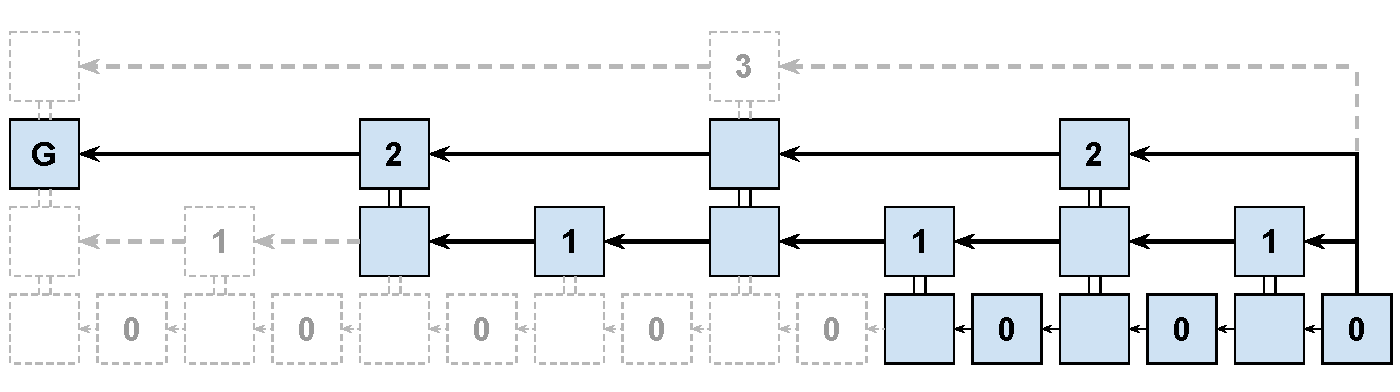
\includegraphics[width=\columnwidth,keepaspectratio]{../chapters/introduction/figures/non-interactive-popow.pdf}
    \label{fig.nipopow-example}
\end{figure}

To compare two proofs $\pi_1$ and $\pi_2$ of this style, the verifier first
finds the LCA block $b$ among them. He then chooses a level $\mu$ such that at
least one of the provers has provided $m$ blocks of level $\mu$ after $b$ and
compares the count of distinct blocks at that level.
Even though multiple levels have been included in the proof, the proofs only
take logarithmic size and are therefore succinct. The reason is that the number
of levels is logarithmic, while the number of blocks included in each level is
constant and approximately $2m$ per level, bringing the total to
$2m\log|\chain|$.
